\chapter{Functions and Expressions}

\section{Expressions}
\begin{itemize}
	\item Call expression anatomy: <Operator>(<Operands>)
	\item Call expressions evaluate to \emph{values}
	\item Order of evaluation:
	\begin{itemize}
		\item Evaluate operator
		\item Evaluate operands
		\item Apply operator function onto operand values
	\end{itemize}
	\item Primitive expressions
	\begin{itemize}
		\item Number: 2
		\item Name: add
		\item String: 'hello'
	\end{itemize}
\end{itemize}

\section{Environment Diagrams}
\medskip
\begin{figure}[H]
  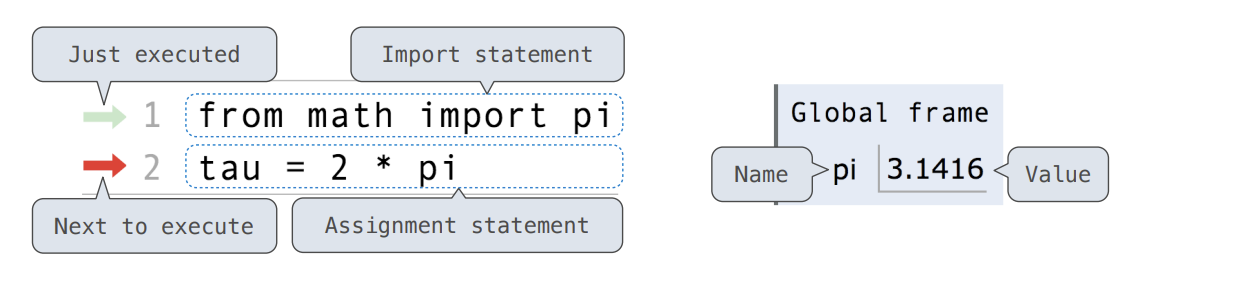
\includegraphics[width=1\linewidth]{figures/environment_diagram.png}
  \caption{Example Environment Diagram}
\end{figure}
\begin{itemize}
	\item Visualization fo the interpreter's process
	\item Left side: statements and expressions
	\begin{itemize}
		\item Arrows indicate evaluation order
	\end{itemize}
	\item Right side: names bounded to values in frames
	\begin{itemize}
		\item Names cannot be repeated in the same frame
		\item An environment in a \emph{sequence of frames}: a frame, its parent frame, and so on
		\item A name evaluates to the value bound to the name in the \emph{earliest frame} of the current environment
		\item Look in the local frame, then in the parent frame, and so on until the global frame
		\item Every expression is evaluated in the context of its environment
	\end{itemize}
	\item Assignment statements: right side is evaluated, and resulting value(s) are binded to the name(s) on the left side
\end{itemize}

\section{Functions}
\begin{itemize}
	\item Function signature anatomy: <name>(<formal parameters>)
	\item Execution order for applying user-defined functions:
	\begin{enumerate}
		\item Create local frame
		\item Bind formal parameters to arguments
		\item Execute the function body in the local frame
	\end{enumerate}
	\item None represents nothing
	\item The return statement completes the evaluation of the call expression
    \item A function that does not explicitly return a value returns None
    \item Pure function: just returns a value
    \item Non-pure function: has side effects
\end{itemize}

\section{Statements}
\begin{itemize}
	\item A statement is \emph{executed by the interpreter to perform an action}
	\medskip
	\begin{figure}[H]
	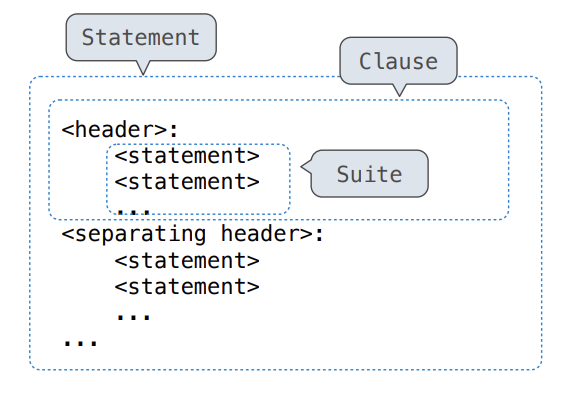
\includegraphics[width=0.5\linewidth]{figures/compound_statement.png}
	\caption{Compound Statement Anatomy}
	\end{figure}
	\item Conditional statement: if clause, followed by elif/else clauses
	\item Execution:
	\begin{enumerate}
		\item Evaluate header expression
		\item If true, execute the suite and skip the remaining clauses
	\end{enumerate}
	\item False values in Python: False, 0, '', None
	\item True values are anything else
	\item While statements (iteration)
	\item Execution:
	\begin{enumerate}
		\item Evaluate header expression
		\item If true, execute the suite and return to step 1
	\end{enumerate}
\end{itemize}